\documentclass[11pt,a4paper]{article}

% --- Packages -----------------------------------------------------------
\usepackage[T1]{fontenc}
\usepackage{lmodern}
\usepackage[margin=2.5cm]{geometry}
\usepackage{amsmath, amssymb}
\usepackage{booktabs}
\usepackage{graphicx}
\usepackage{array}
\usepackage{enumitem}
\usepackage{xcolor}
\usepackage[hidelinks,colorlinks=true,linkcolor=blue!50!black,citecolor=blue!50!black,urlcolor=blue!50!black]{hyperref}
\usepackage[numbers,sort&compress]{natbib}
\usepackage{authblk}

% --- Custom commands ----------------------------------------------------
\newcommand{\HFF}{\textsc{hff}}
\newcommand{\Chandra}{\textit{Chandra}}
\newcommand{\Xres}{X_{\mathrm{res}}}
\newcommand{\Vobs}{V_{\mathrm{obs}}}
\newcommand{\Vnull}{V_{\mathrm{null}}}
\newcolumntype{L}[1]{>{\raggedright\arraybackslash}p{#1}}

% --- Title --------------------------------------------------------------
\title{A Controlled Lensing/X-ray Cross-Readout Enrichment Audit in HFF and CLASH Clusters}

\author[1]{J\'ozsef Olcs\'ak}
\affil[1]{Independent researcher, Budapest, Hungary}

\date{Internal draft v0 --- 2026-05-21\\Last revised: 2026-08-22}

\begin{document}

\maketitle

\begin{abstract}\sloppy
We present a controlled X-ray/lensing enrichment audit for six Hubble Frontier
Fields strong-lensing clusters and a frozen external CLASH map-level
validation sample. For each system we compare radius- and exposure-controlled
\Chandra{} X-ray structure against public convergence and magnification maps.
The primary statistic is top-region enrichment relative to matched null
controls, used here as a cross-readout enrichment diagnostic. In the \HFF{}
development sample, all six clusters have median residual/null ratios above
unity, and 88 of 92 tested model/observable/tracer rows are above their
matched-null mean. In the external CLASH validation sample, 12 non-\HFF{}
clusters pass the frozen population endpoint: a spatial-block-aware
hierarchical fit gives a population residual/null ratio of 1.231 with an
approximate 95 percent interval of 1.119--1.353. However, weak and below-null
magnification/residual channels remain in the row table. We therefore
interpret the result as a model-sensitive observational enrichment statistic,
not as a universal lensing-readout law, a final physical field, a derived
mechanism, or a dark-matter replacement proof.
\end{abstract}

\tableofcontents

\section{Introduction}

Cluster lensing analyses compare several imperfect readouts of the same
projected system: reconstructed convergence, magnification, X-ray structure,
galaxy light, and model-family assumptions. This paper asks a deliberately
narrow question about those readouts. It does not try to solve the mass-tracer
gap by introducing a new hidden component. The useful question is narrower and
falsifiable:
\begin{quote}
Can controlled lensing/X-ray cross-readout enrichment be detected without
adding a fitted hidden density component?
\end{quote}

This draft studies that question using Hubble Frontier Fields lensing maps and
\Chandra{} X-ray structure. The goal is not to derive a physical mechanism.
The goal is to define and test an observational prefilter:
\begin{quote}
Do controlled X-ray residual structures preferentially lie inside high
lensing-readout regions above matched geometry-preserving nulls?
\end{quote}

\subsection{Source-transport boundary}

The present enrichment statistic compares terminal observational maps. It
does not reconstruct a smooth optical source arrow, a body connection, or an
observer--source transport law. In the current Tau Core source ledger, a
non-scalar smooth optical transport can arise without a fitted gain only from
one of two independently supplied structures: holonomy of a full body
connection, or Kato transport of a varying, constant-rank, source-owned access
projector, with generator \([dP_O,P_O]\). A scalar phase connection may carry
clock or phase information, but it cannot determine normalized non-scalar
optical orientation. Consequently, a positive value of
Eq.~\eqref{eq:visibility} remains a cross-readout association and cannot by
itself identify either optical source mechanism.

\section{Observational Hypothesis}

Let
\begin{equation}
\Xres = \text{Chandra X-ray structure after radius and exposure controls}
\end{equation}
and let $L$ be a declared \HFF{} lensing readout, either convergence $\kappa$ or
magnification $\mu$. The cross-readout enrichment hypothesis predicts
\begin{equation}
\Vobs(L,\Xres) > \Vnull(L,\Xres),
\label{eq:visibility}
\end{equation}
where $\Vobs$ is top-region enrichment and $\Vnull$ is the matched-null
expectation. Equation~\ref{eq:visibility} is a screening diagnostic, not a
field equation. It is only meaningful after declaring the cluster, model
family, observable channel, tracer definition, and control family. This
prevents the claim from becoming a post-hoc statement that any attractive
overlap between any two maps supports a preferred physical theory.

\section{Data and Provenance}

The development analysis uses public \HFF{} lens-model products and
\Chandra{} X-ray products. The lensing side includes the \HFF{} model families
available in the local input set: Merten, CATS, Diego, and Williams. The
development cluster sample is Abell S1063, Abell 2744, Abell 370, MACS0416,
MACS0717, and MACS J1149.5+2223.

The external validation sample uses public CLASH lensing products and archived
\Chandra{} data. Before inspecting the external endpoint, the branch froze a
12-cluster non-\HFF{} CLASH sample: RX J1347.5-1145, MACS J2129.4-0741, MACS
J1206.2-0847, CL J1226.9+3332, MS 2137.3-2353, MACS J1423.8+2404, Abell 2261,
MACS J1311.0-0310, MACS J1931.8-2635, RX J1532.9+3021, MACS J0744.9+3927, and
MACS J0329.7-0211. The external map-level runner uses Zitrin LTM-Gauss and
Zitrin NFW CLASH convergence and magnification products, paired with uniform
\Chandra{} broad-band flux/exposure products reduced in the local CIAO
pipeline~\citep{mast_clash_hlsp,zitrin2014_clash_lensing_models}.

The \HFF{} lens-model archive and published model-comparison references are
treated as the current bibliography scaffold~\citep{stsci_hff_lensmodels,
johnson2014_hff_lens_models,jauzac2014_hff_mass_magnification_maps,
meneghetti2017_frontier_fields_lens_modelling_comparison,
priewe2017_lens_models_under_microscope}. The software layer uses the
Astropy ecosystem~\citep{astropy2013,astropy2018,astropy2022},
reprojection tooling~\citep{reproject_package}, and \Chandra{}/CXC resources
\citep{ciao_cxc_citation}. The local paper branch includes a README-level
model-product audit covering the method-family citation keys for SaWLens,
LENSTOOL/CATS, WSLAP+, and GRALE. Before submission, those method references
must receive a final publisher/ADS metadata check and exact acknowledgement
text.

\section{Methods}

The paper-facing controlled tracer is
\begin{equation}
\Xres = \texttt{chandra\_xray\_radius\_exposure\_residual\_z}.
\end{equation}

For each cluster, model family, and lensing observable, the runner measures
\begin{equation}
E_{\mathrm{obs}}
 =
 \frac{
   \mathrm{fraction}(\mathrm{top}\ L\ \mathrm{inside}\ \mathrm{top}\ \Xres)
 }{
   \mathrm{base\ fraction}(\mathrm{top}\ \Xres)
 }.
\end{equation}

The paper-facing diagnostic ratio is
\begin{equation}
R_{\mathrm{null}} =
\frac{E_{\mathrm{obs}}}{\langle E_{\mathrm{null}}\rangle}.
\label{eq:nullratio}
\end{equation}
Values above unity indicate excess relative to the declared null. Values below
unity are retained as weak or null channels.

\section{Results}

Across the all-six first-pass runner table, 92 model/observable/tracer rows are
tested. Of these, 88 are above matched null and four are below matched null. At
cluster level, all six systems have median residual/null ratios above unity:
Abell S1063, Abell 2744, Abell 370, MACS0416, MACS0717, and MACS
J1149.5+2223. Four clusters have every tested row above unity; Abell 370 and
MACS0717 retain channel-level falsifiers.

\begin{figure}[p]
\centering
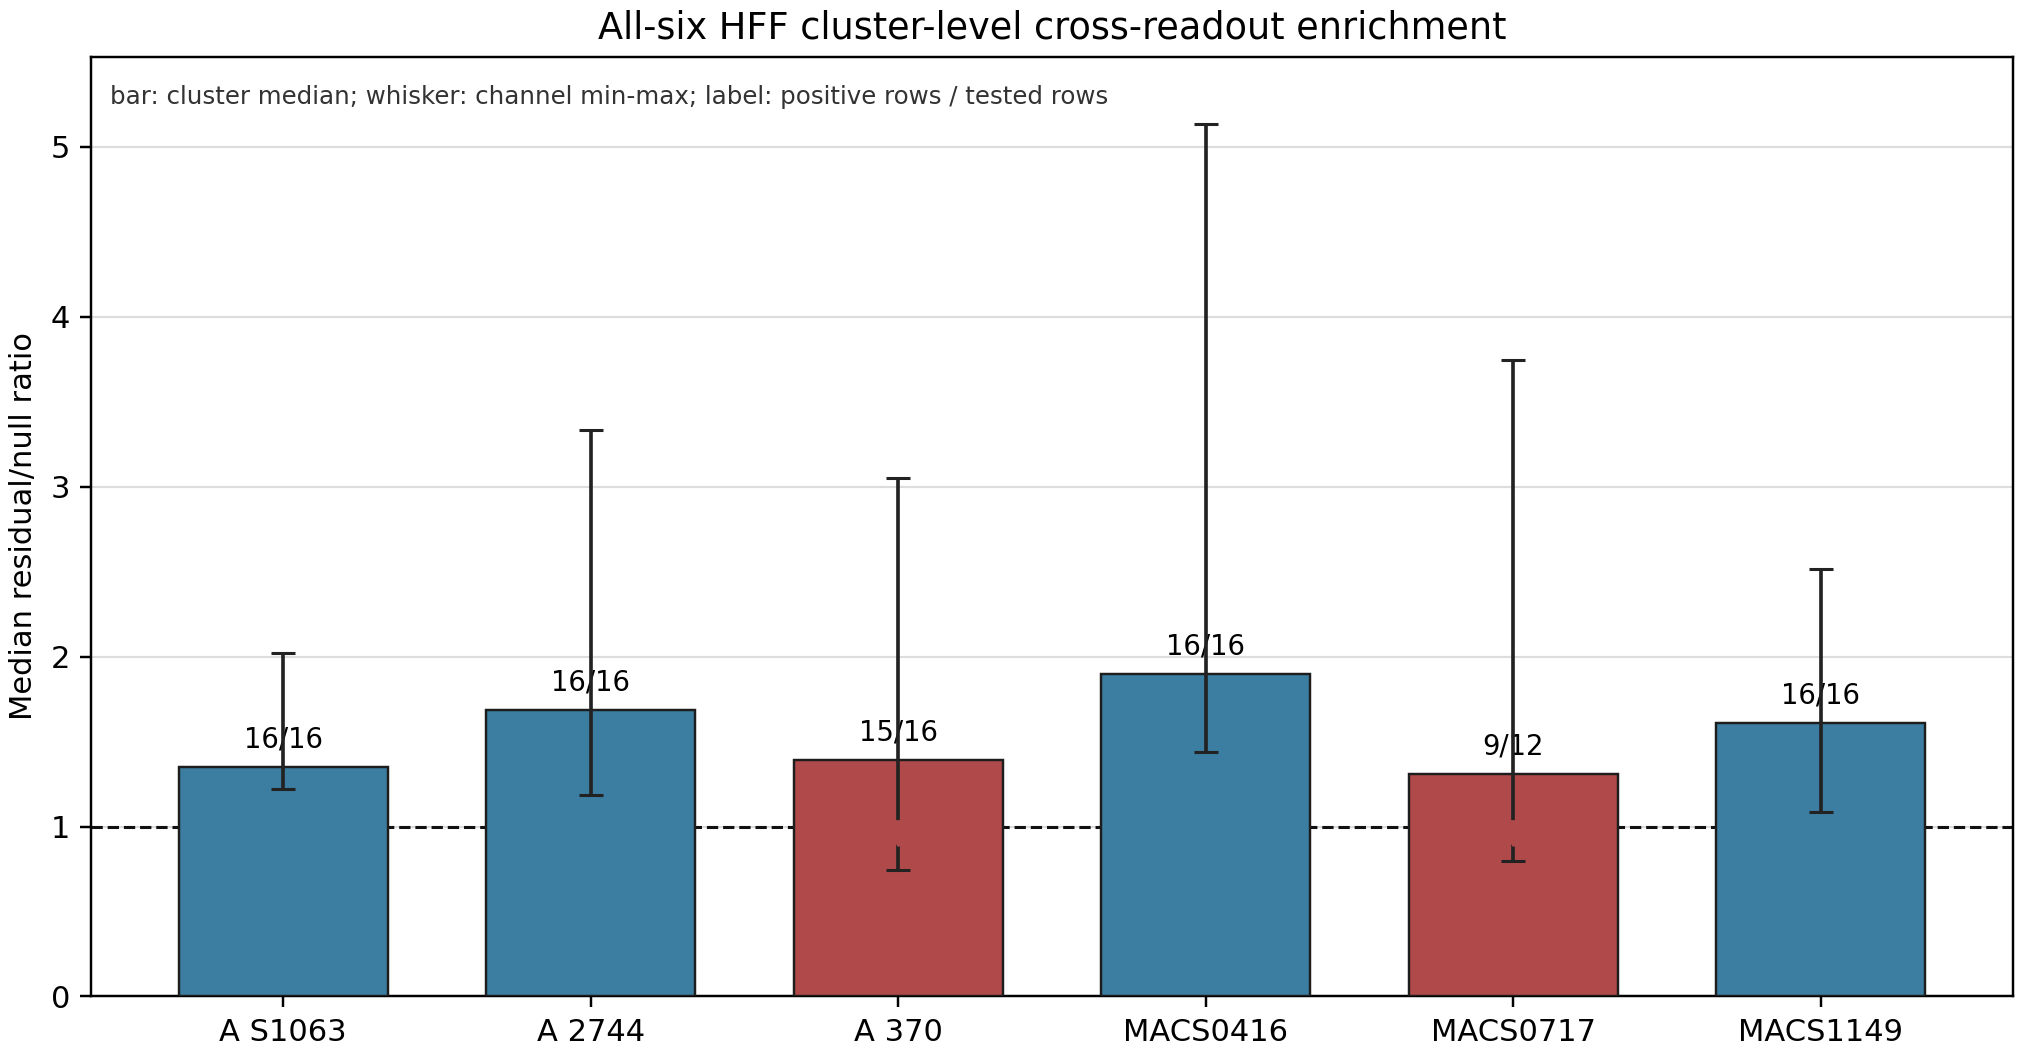
\includegraphics[width=0.92\textwidth]{figures/all_six_cluster_meta_summary_v1.png}
\caption{All-six \HFF{} cluster-level cross-readout enrichment summary. Bars
show the median observed/matched-null ratio across predeclared
model/observable/tracer rows for each cluster; whiskers show the within-cluster
channel minimum and maximum. Text labels report positive rows over tested
rows. Red markers indicate clusters with retained below-null channels. This is
the preferred paper-facing summary because the cluster, not the pixel or row,
is the exploratory unit.}
\label{fig:all-six-meta}
\end{figure}

The retained below-null rows are:
\begin{center}
\begin{tabular}{llllr}
\toprule
Cluster & Model & Observable & Tracer & $R_{\mathrm{null}}$ \\
\midrule
Abell 370 & Williams v4.1 & magnification & X-ray $\sigma_1$ & 0.744 \\
MACS0717 & Williams v4.1 & magnification & X-ray $\sigma_1$ & 0.797 \\
MACS0717 & Williams v4.1 & magnification & X-ray residual & 0.873 \\
MACS0717 & Diego v4.1 & magnification & X-ray $\sigma_1$ & 0.894 \\
\bottomrule
\end{tabular}
\end{center}

\begin{figure}[p]
\centering
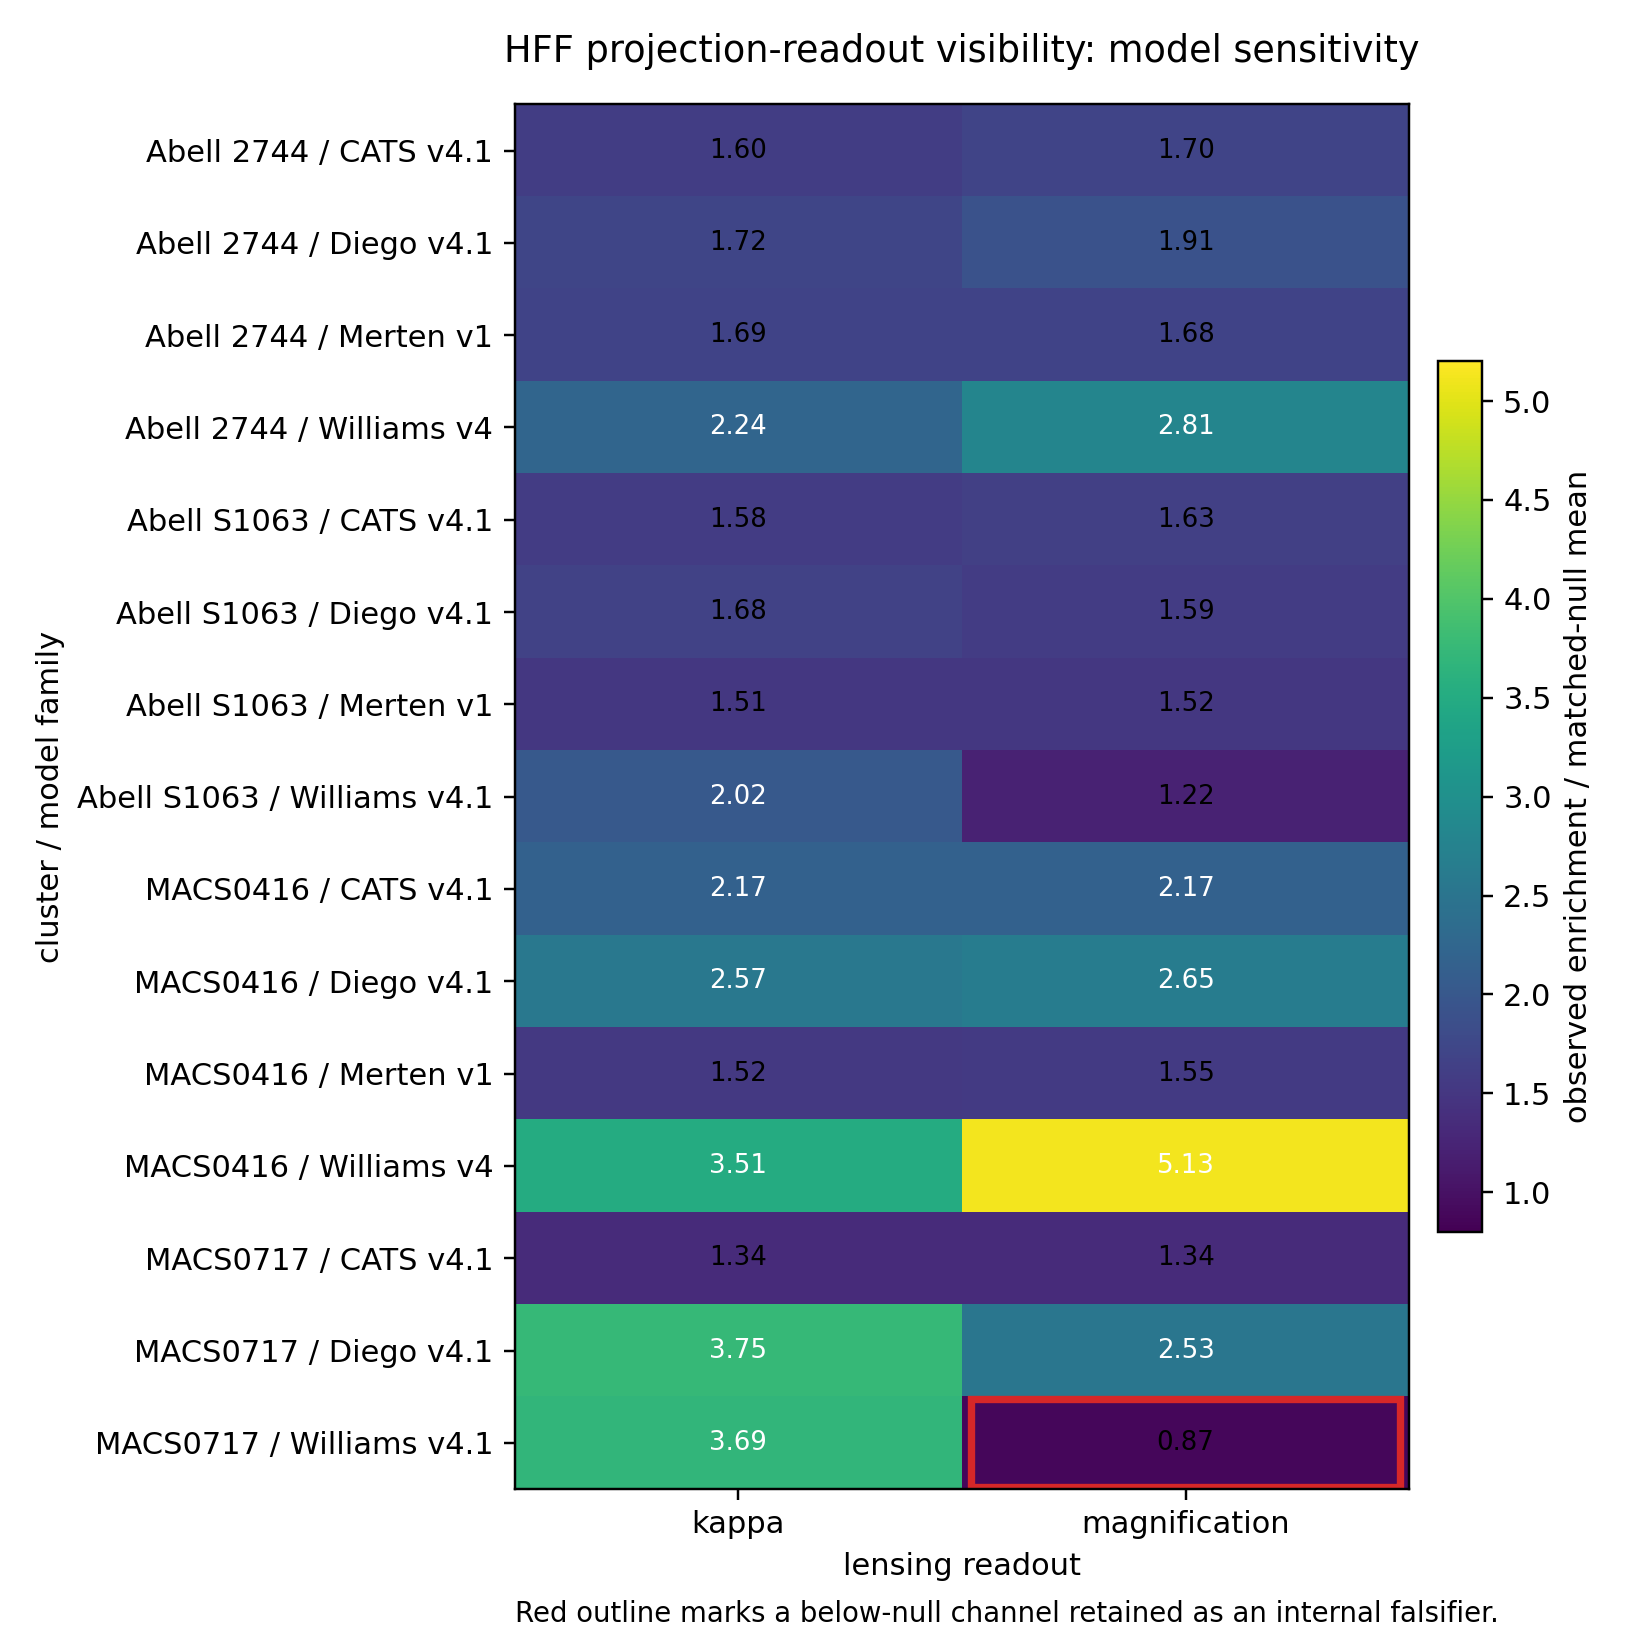
\includegraphics[width=0.82\textwidth]{figures/model_sensitivity_heatmap_v1.png}
\caption{Model-sensitivity of \HFF{} cross-readout enrichment. Each
entry reports the ratio between observed enrichment and the matched-null mean
for the controlled \Chandra{} radius+exposure residual tracer in the original
four-cluster paper-facing sensitivity table. Values above unity indicate excess
co-location relative to the declared null. The MACS0717 Williams magnification
entry is below unity and is retained as an internal falsifier.}
\label{fig:sensitivity}
\end{figure}

\begin{figure}[p]
\centering
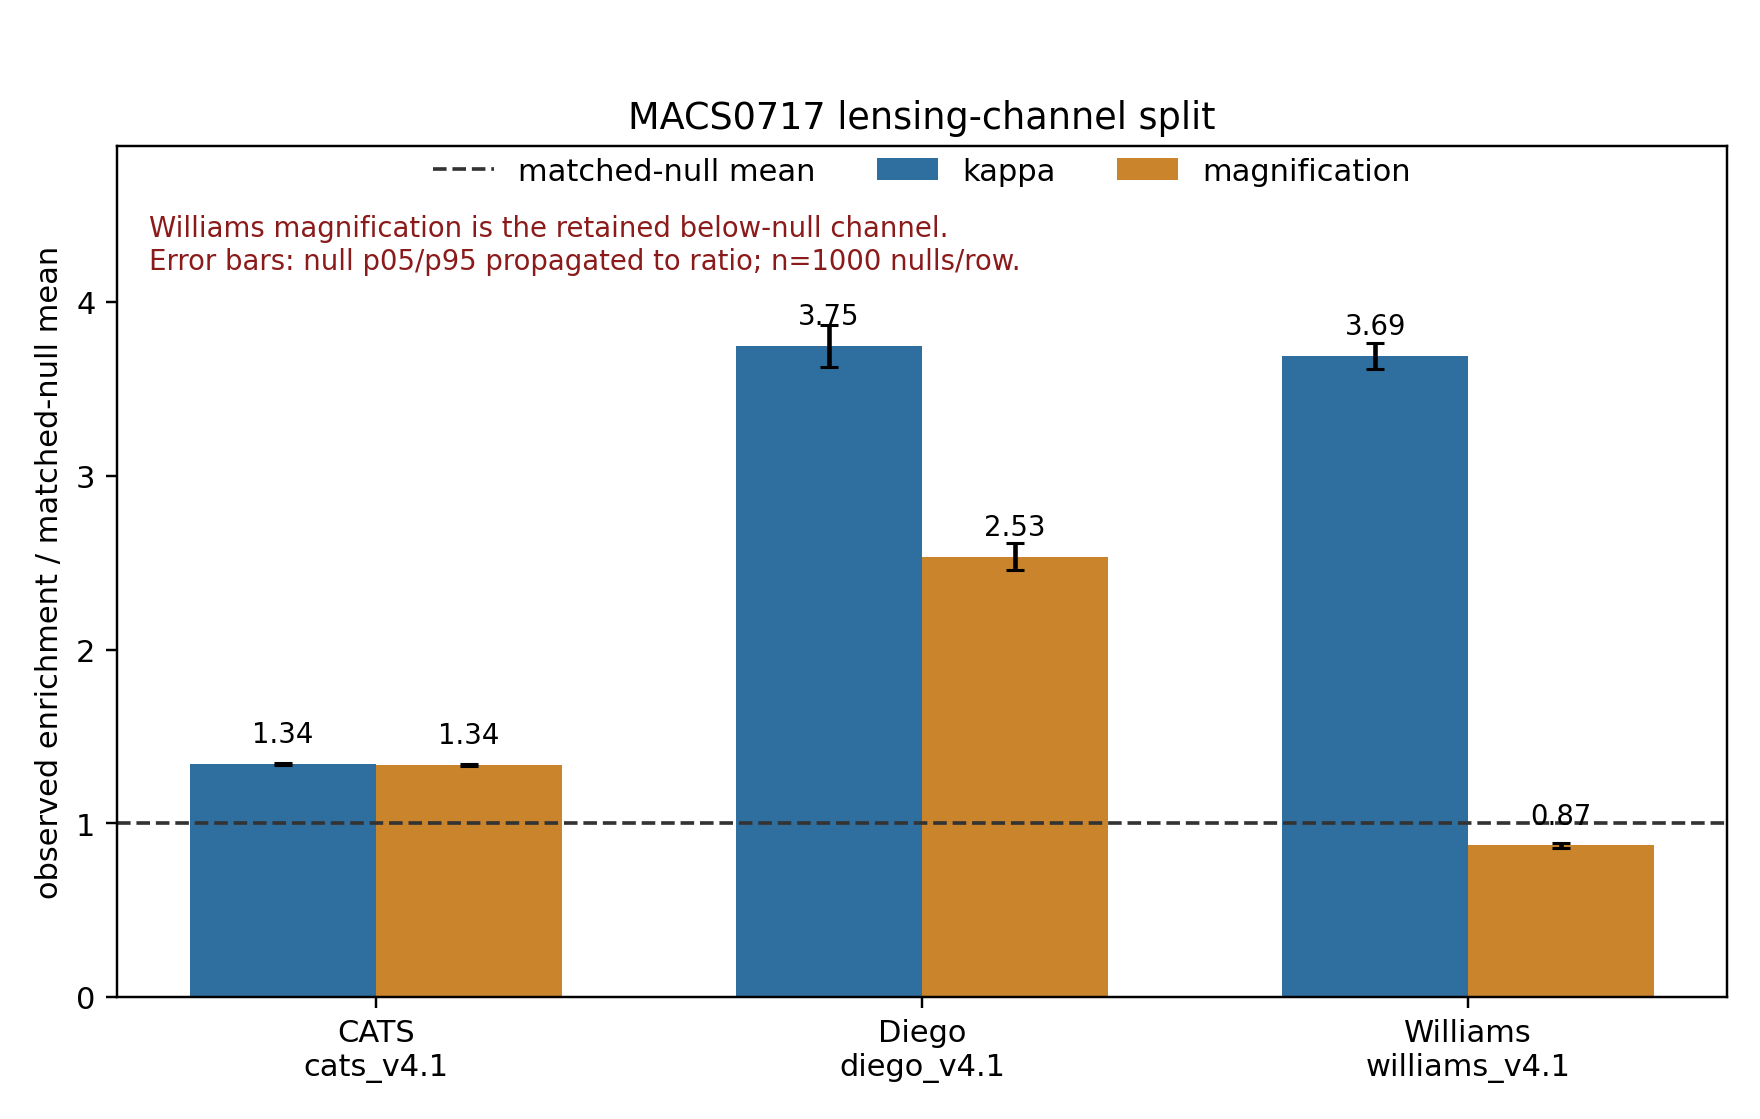
\includegraphics[width=0.82\textwidth]{figures/macs0717_channel_split_v1.png}
\caption{MACS0717 lensing-channel split. CATS and Diego are positive in both
convergence and magnification. Williams convergence is positive, while
Williams magnification falls below matched null. Error bars propagate the
matched-null p05/p95 interval to the displayed observed/null ratio, with
$n=1000$ null samples per row. This demonstrates that the observed enrichment
pattern is channel-sensitive and cannot be stated as a universal property
of all lensing products.}
\label{fig:macs0717}
\end{figure}

In the original four-cluster residual-only table, the below-null channel is:
\begin{align}
E_{\mathrm{obs}} &= 0.945,\\
\langle E_{\mathrm{null}}\rangle &= 1.083,\\
R_{\mathrm{null}} &= 0.873,
\end{align}
for MACS0717 Williams magnification, with empirical $p(\geq E_{\mathrm{obs}})=1.000$.
This is not a nuisance row to hide. It is an internal falsifier.

\section{Negative Controls}

The negative-control summary uses roll and value-shuffle controls. The control
ratios are generally above unity, supporting the interpretation that the signal
is not merely a baseline top-region occupancy effect. Weak control rows remain
and should be preserved as scope limits, especially for MACS0717 magnification
and selected Abell 2744 control minima.

\begin{figure}[p]
\centering
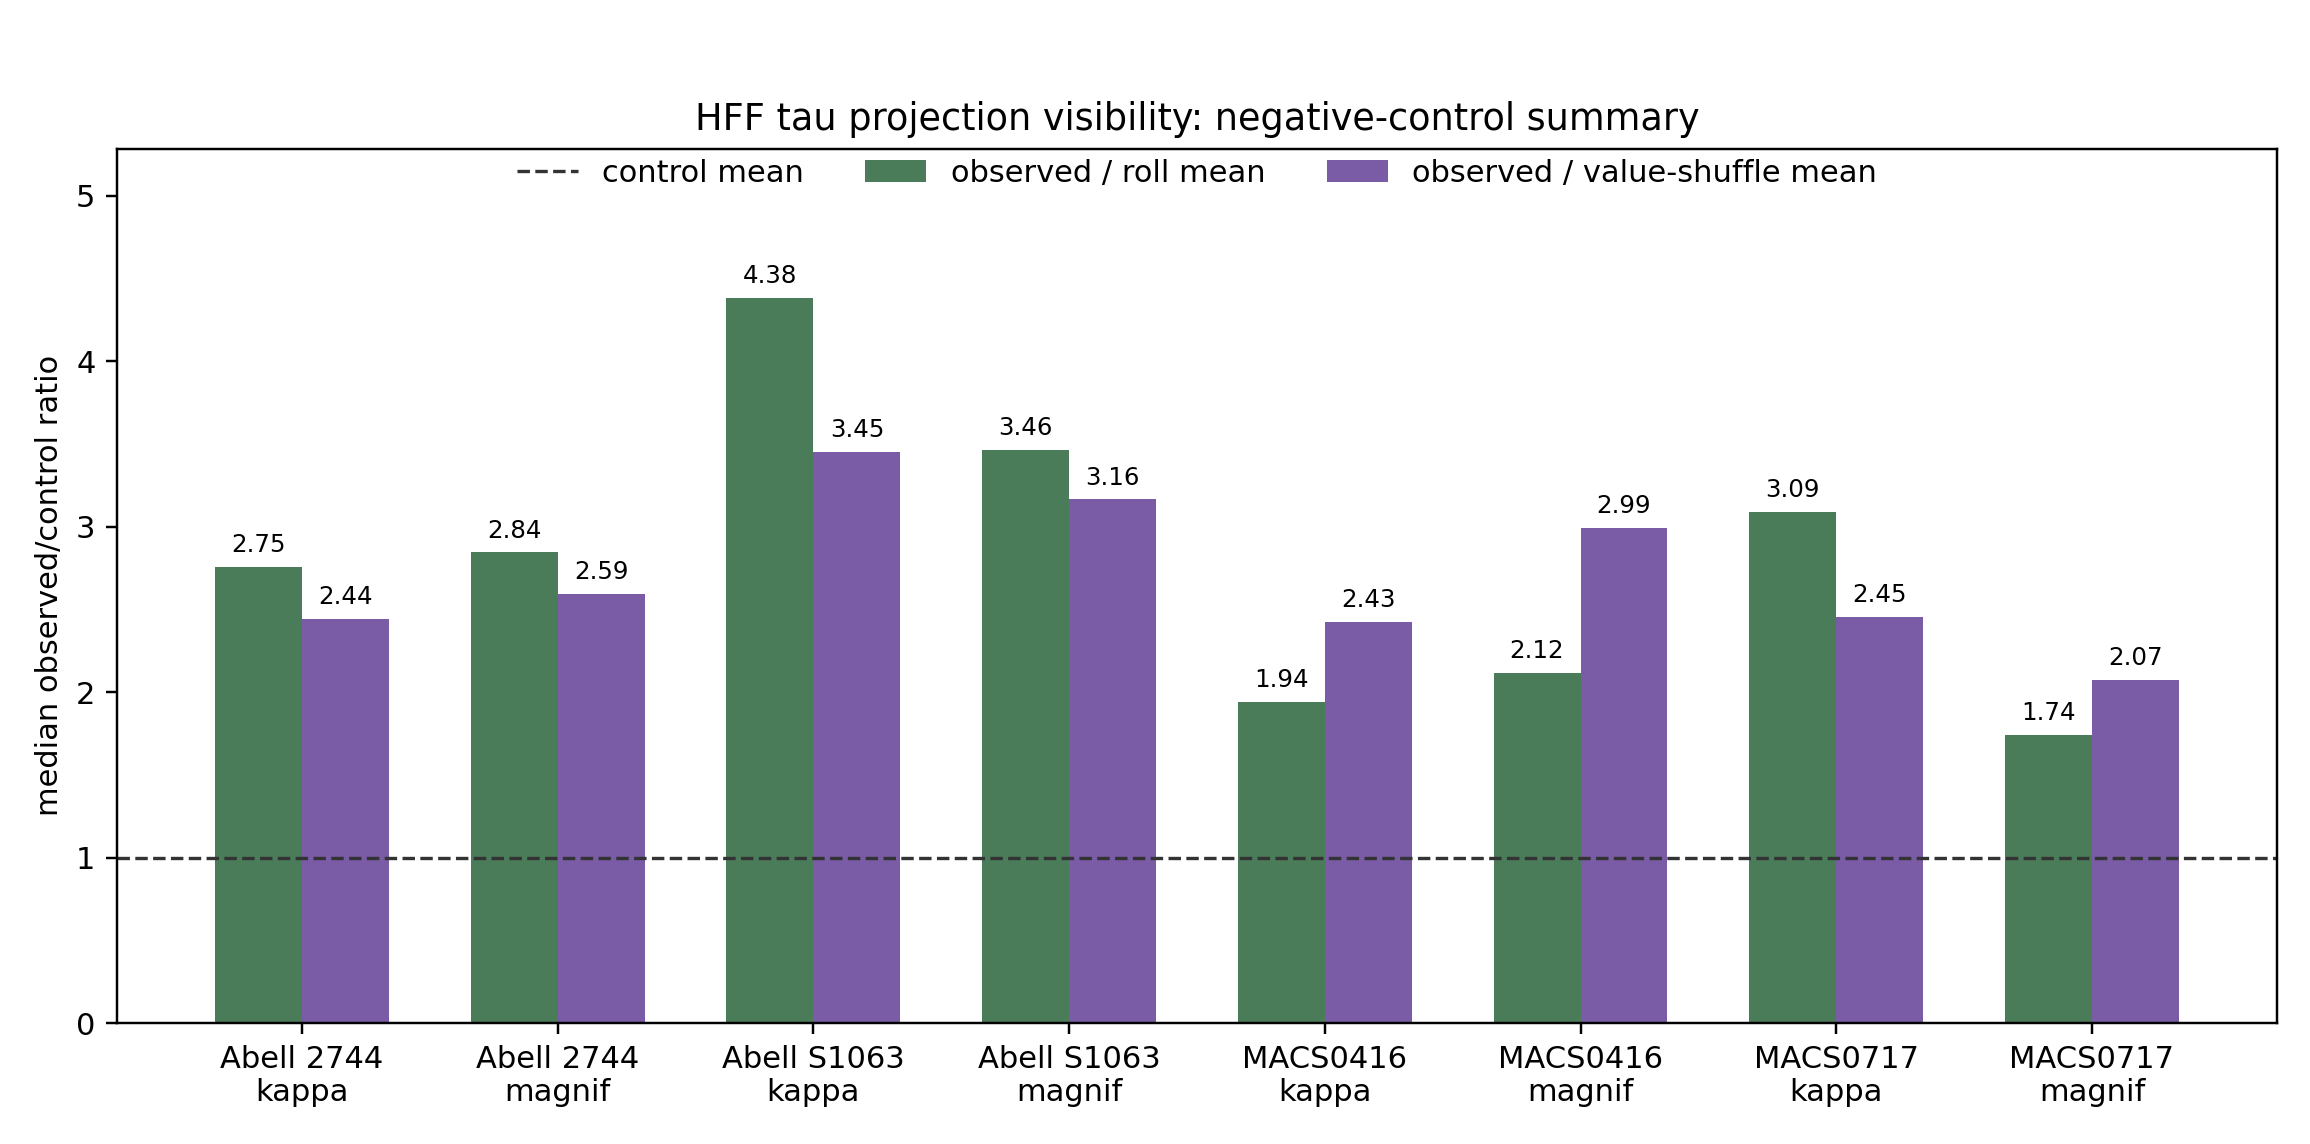
\includegraphics[width=0.92\textwidth]{figures/negative_control_summary_v1.png}
\caption{Negative-control summary. Bars show median observed/control ratios
for roll and value-shuffle controls, grouped by cluster and lensing observable.
The dashed line marks the control mean.}
\label{fig:negative-controls}
\end{figure}

\section{Statistical Hardening Status}

The current statistics support an exploratory enrichment screen, not a
population-level detection. In the all-six first-pass runner table, the
matched-null summaries use 1000 null samples per row. Of 92 rows, 88 are above
the matched-null mean and 88 are above the matched-null 95th percentile. The
four retained below-null rows are all magnification-channel failures: one in
Abell 370 and three in MACS0717. This is a model/readout sensitivity result, not
a row to hide.

This is stronger than a visual-overlap claim, but it is still not a complete
publication-grade uncertainty model. The next statistical hardening layer must
add bootstrap confidence intervals on effect sizes, uncertainty bands on
$R_{\mathrm{null}}$, spatial-autocorrelation-aware resampling, grouped
multiple-hypothesis correction by cluster/model/channel family, and an explicit
treatment of lens-model reconstruction covariance. Until those are complete,
the correct language is exploratory enrichment screen rather than strong
statistical detection.

The spatial-autocorrelation issue is the most important remaining technical
limitation. Cluster maps are smoothed and neighboring pixels are not
independent, so the effective degrees of freedom can be much smaller than the
pixel count. A publication-grade detection claim would require at minimum a
spatial block bootstrap, annulus-preserving block shuffles, a correlation-length
sweep, and a cluster-level meta-analysis in which the six clusters, not the
pixels, are the independent units.

At the current cluster level, all six \HFF{} systems have median
cross-readout enrichment above matched null. Four of the six clusters have
all tested rows above unity; Abell 370 and MACS0717 retain specific below-null
magnification channels. This cluster-level summary is more
appropriate than treating all pixels or rows as independent detections, but it
does not overcome the small-sample limitation.

\section{Compact-Source Masking}

Compact-source masking addresses a simple contamination explanation: that the
visibility signal is driven by a small number of compact X-ray peaks rather than
cluster-scale morphology. For the original four-cluster audit we compare the
unmasked X-ray/lensing enrichment to a strict compact mask (``compact p99,
dilation 2''). The covered rows all survive this stress test: the minimum
masked/unmasked enrichment ratio is 1.018. MACS0717 additionally retains
annulus-preserving radial-null support under the same strict mask.

\begin{figure}[p]
\centering
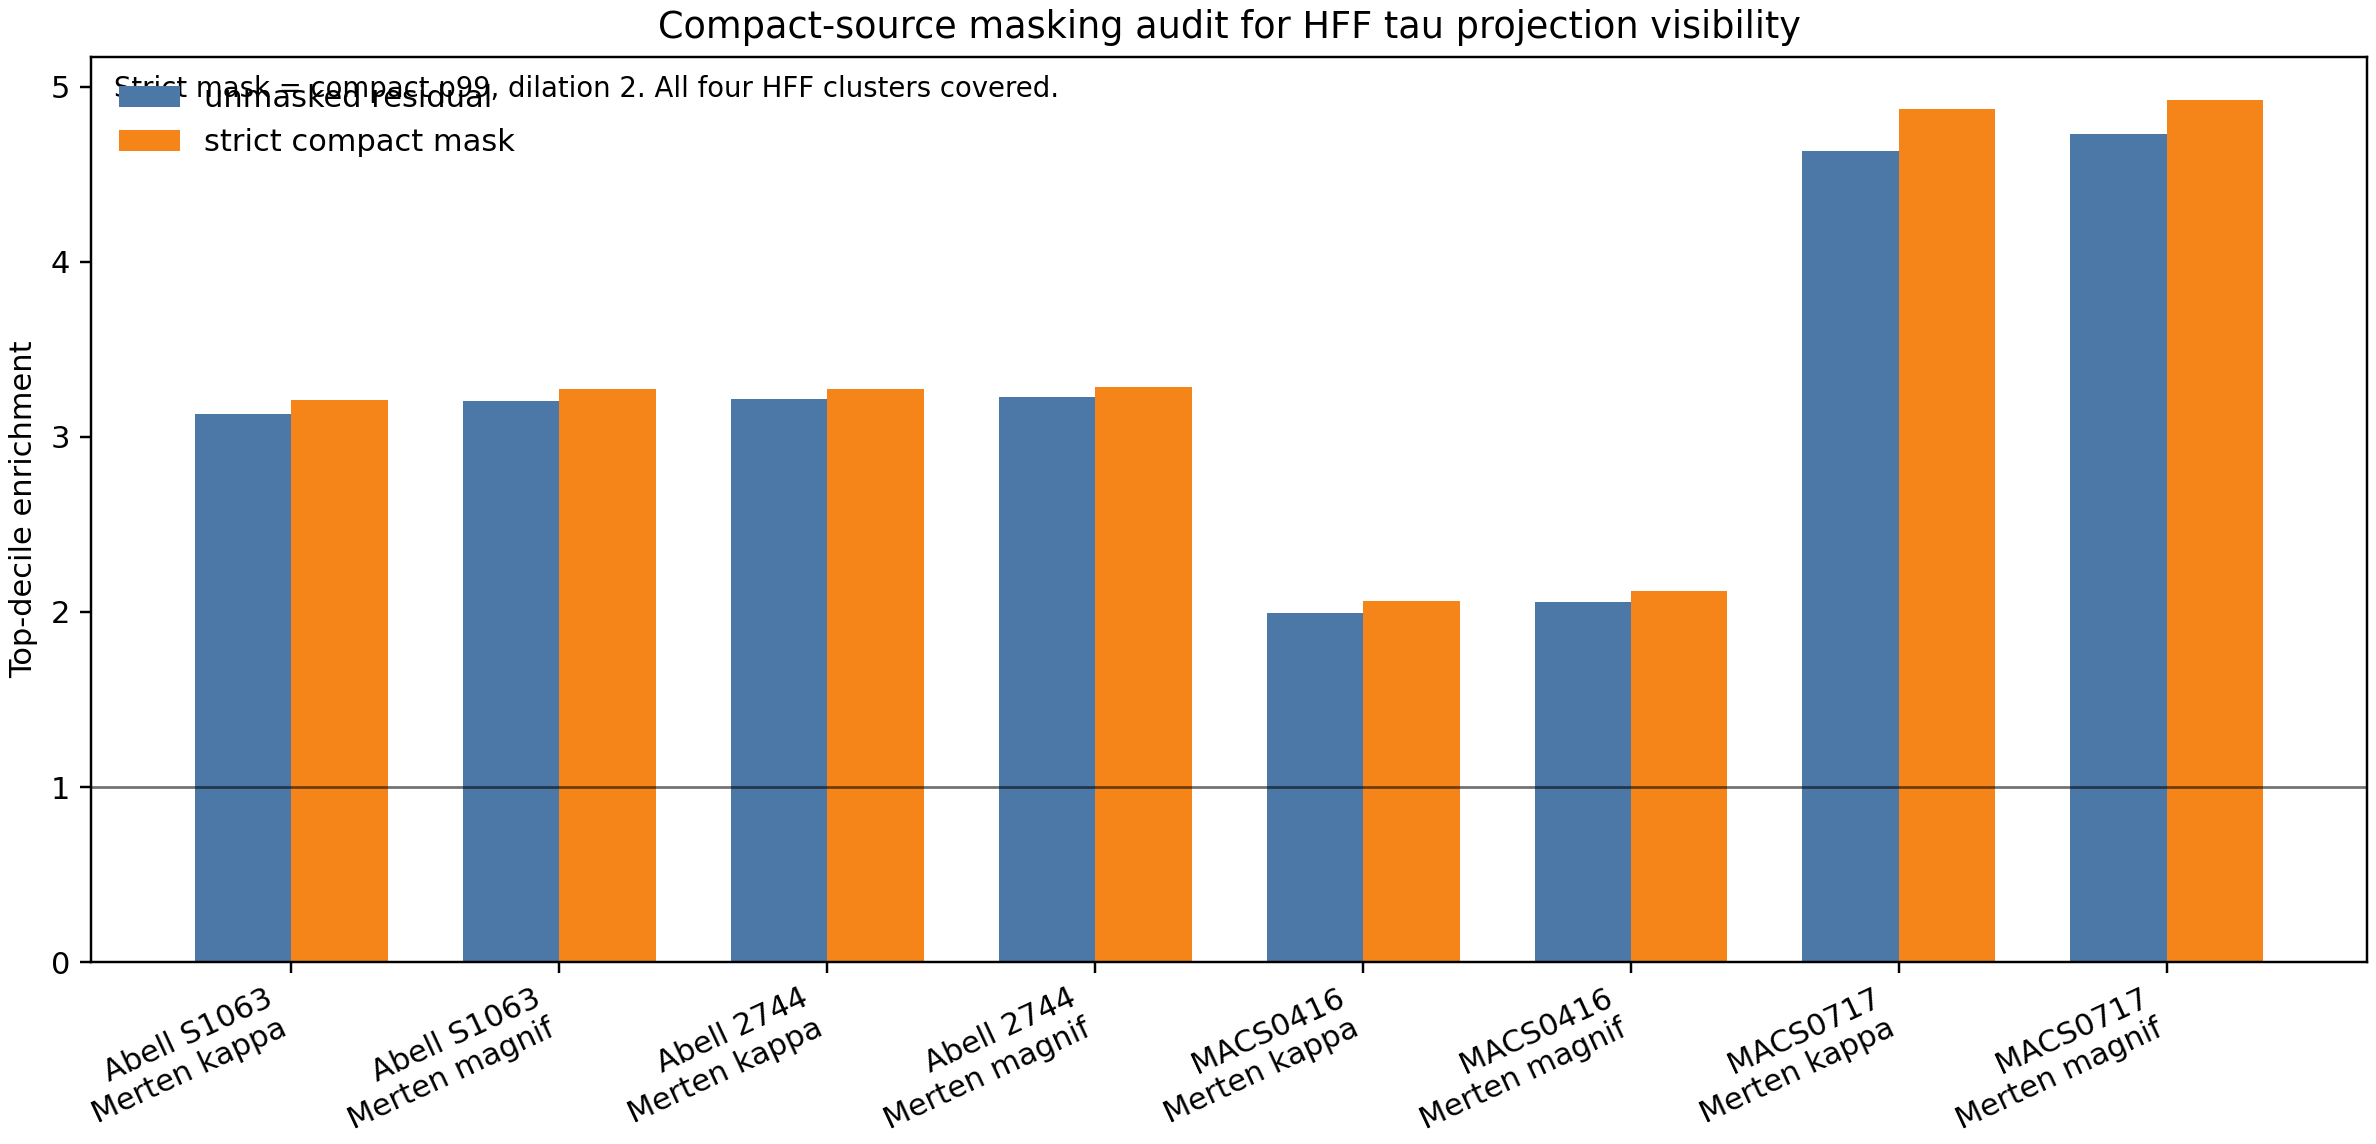
\includegraphics[width=0.90\textwidth]{figures/compact_source_masking_audit_v1.png}
\caption{Compact-source masking audit. Bars compare unmasked and strict
compact-masked X-ray/lensing enrichment for the covered clusters. The test does
not prove a physical mechanism, but it argues against the simplest compact
X-ray-peak contamination explanation for the enrichment statistic.}
\label{fig:compact-source}
\end{figure}

\section{Model-Family Uncertainty}

The candidate-map weight is a mean of independent \HFF{} kappa percentile-rank
maps. A mean map is useful, but it can hide disagreement among lens-model
families. We therefore generate a companion uncertainty layer: mean kappa-rank,
pixelwise kappa-rank scatter, and the fraction of model families that place a
pixel in their top-rank support. The median cluster-level kappa-rank scatter is
0.186, and the largest cluster-level 90th-percentile scatter is 0.382. MACS0717
has the largest median scatter among the original four systems, consistent with the
channel sensitivity already exposed by the Williams magnification falsifier.

\begin{figure}[p]
\centering
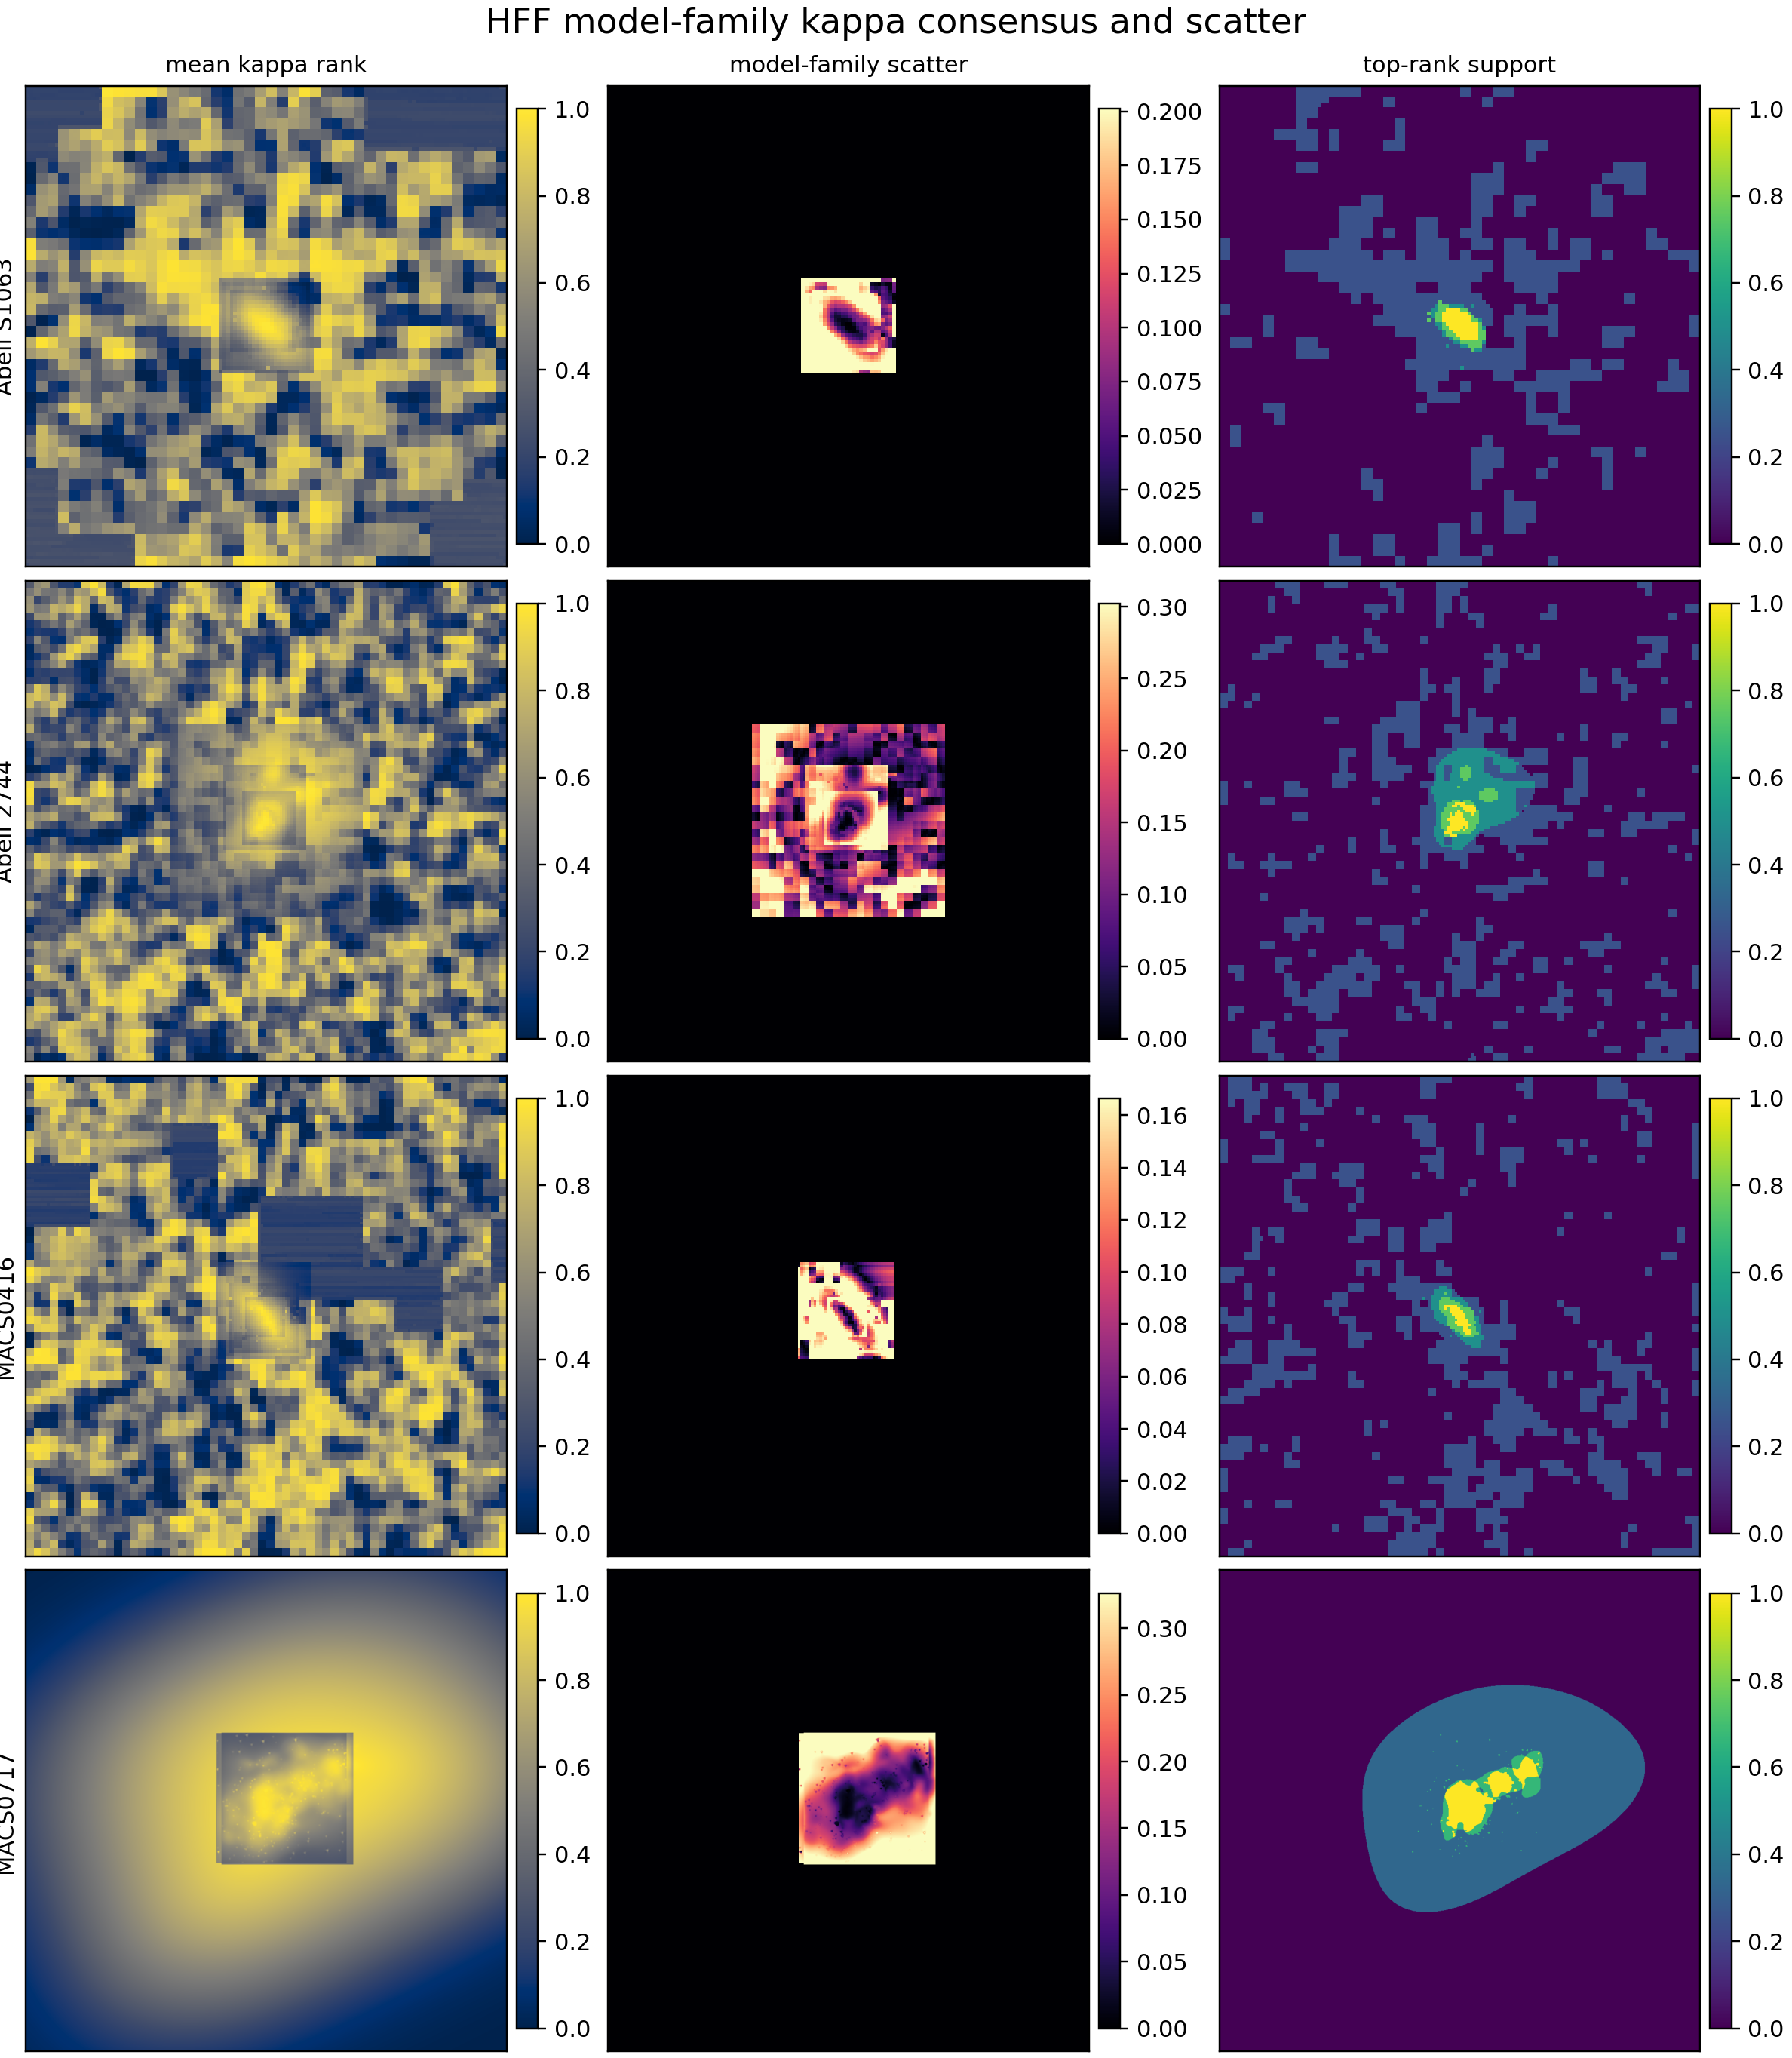
\includegraphics[width=0.92\textwidth]{figures/model_family_uncertainty_panel_v1.png}
\caption{Model-family kappa consensus and scatter. The left column shows mean
kappa percentile-rank support, the middle column shows pixelwise scatter across
available model families, and the right column shows top-rank support fraction.
This panel is an honesty layer for the candidate visibility maps: high mean
support should be read together with model-family scatter.}
\label{fig:model-family-uncertainty}
\end{figure}

\section{Conventional Explanations}

A positive X-ray/lensing enrichment pattern is not automatically evidence for a
new physical mechanism. Several conventional explanations can produce
co-location between X-ray residual structure and lensing readouts. Cluster
merger geometry can align shocked or displaced gas with projected potential
features. Baryon--potential alignment can make X-ray morphology and convergence
high points trace the same underlying cluster structure. Hydrostatic or
quasi-hydrostatic gas structure can correlate X-ray brightness with the
gravitational potential even when the system is not fully relaxed. More
generally, X-ray and lensing maps are both expected to co-trace aspects of the
same projected mass distribution.

The lensing products themselves also introduce baseline explanations.
Reconstruction covariance, smoothing scale, model-family priors, and
mass-concentration coupling can move high-rank convergence or magnification
support toward the same cluster-scale features. These are not nuisance details;
they are part of the null hypothesis that the audit must compete against.

\begin{center}
\begin{tabular}{L{0.22\textwidth}L{0.31\textwidth}L{0.35\textwidth}}
\toprule
Baseline & What it can explain & What remains after this audit \\
\midrule
Cluster merger geometry &
Projected merger axes can align gas structure, galaxies, and lensing support. &
The statistic is still tested against radius/exposure and matched spatial
nulls, but merger state is not yet an explicit covariate. \\
Baryon--potential co-tracing &
Gas and lensing can both follow the same large-scale potential. &
This may explain part of the positive enrichment; the audit asks whether the
top-region excess survives declared controls, not whether co-tracing exists. \\
Hydrostatic or quasi-hydrostatic structure &
X-ray brightness can correlate with the gravitational potential in relaxed or
partly relaxed systems. &
The residual tracer subtracts radius/exposure structure, but it does not yet
fit a full thermodynamic cluster model. \\
Reconstruction covariance and smoothing &
Lens-model regularization can broaden or shift high-rank support toward common
cluster-scale features. &
Model-family and channel sensitivity are retained explicitly; this is why
below-null magnification rows are not removed. \\
Source masking and compact peaks &
Point sources or compact gas peaks can create artificial top-region overlap. &
Compact-source checks reduce the simplest contamination story, but a uniform
public mask release remains future work. \\
\bottomrule
\end{tabular}
\end{center}

The present analysis addresses only part of this conventional baseline. Radius
and exposure controls reduce simple radial and instrumental explanations.
Roll/value-shuffle controls reduce generic top-region occupancy explanations.
Compact-source masking reduces the simplest X-ray point-peak contamination
story. Model-family scatter exposes where the lensing readout is unstable.
However, the analysis does not yet fully model merger state, hydrostatic
structure, lensing reconstruction covariance, or smoothing-induced alignment.
For this reason the result should be read as a controlled enrichment pattern
that survives several simple baselines, not as proof that conventional cluster
morphology has been exhausted.

This framing also defines what would make the result less interesting. If a
future baseline model using merger-state covariates, gas thermodynamic
structure, and lensing reconstruction covariance reproduces the same
cluster-level and channel-level enrichment pattern, then the present statistic
should be interpreted as a compact morphology diagnostic rather than evidence
for a new physical readout. Conversely, if the enrichment remains
positive after those baselines are modeled and preregistered on a larger
external sample, then it becomes a stronger constraint on any later physical
interpretation. The current paper deliberately stops at the first statement:
the enrichment survives the controls implemented here, but conventional
cluster morphology remains an active competing explanation.

\section{Candidate Visibility Maps}

Candidate maps were generated as proxy products:
\begin{equation}
T_{\mathrm{Chandra}} =
\max\left(0, \mathrm{robust}\ z(\text{Chandra residual after radius/exposure grouping})\right),
\end{equation}
and
\begin{equation}
T_{\mathrm{vis}} =
T_{\mathrm{Chandra}}\,
\left\langle \mathrm{percentile\ rank}(\kappa_{\mathrm{HFF}}) \right\rangle.
\end{equation}

\begin{figure}[p]
\centering
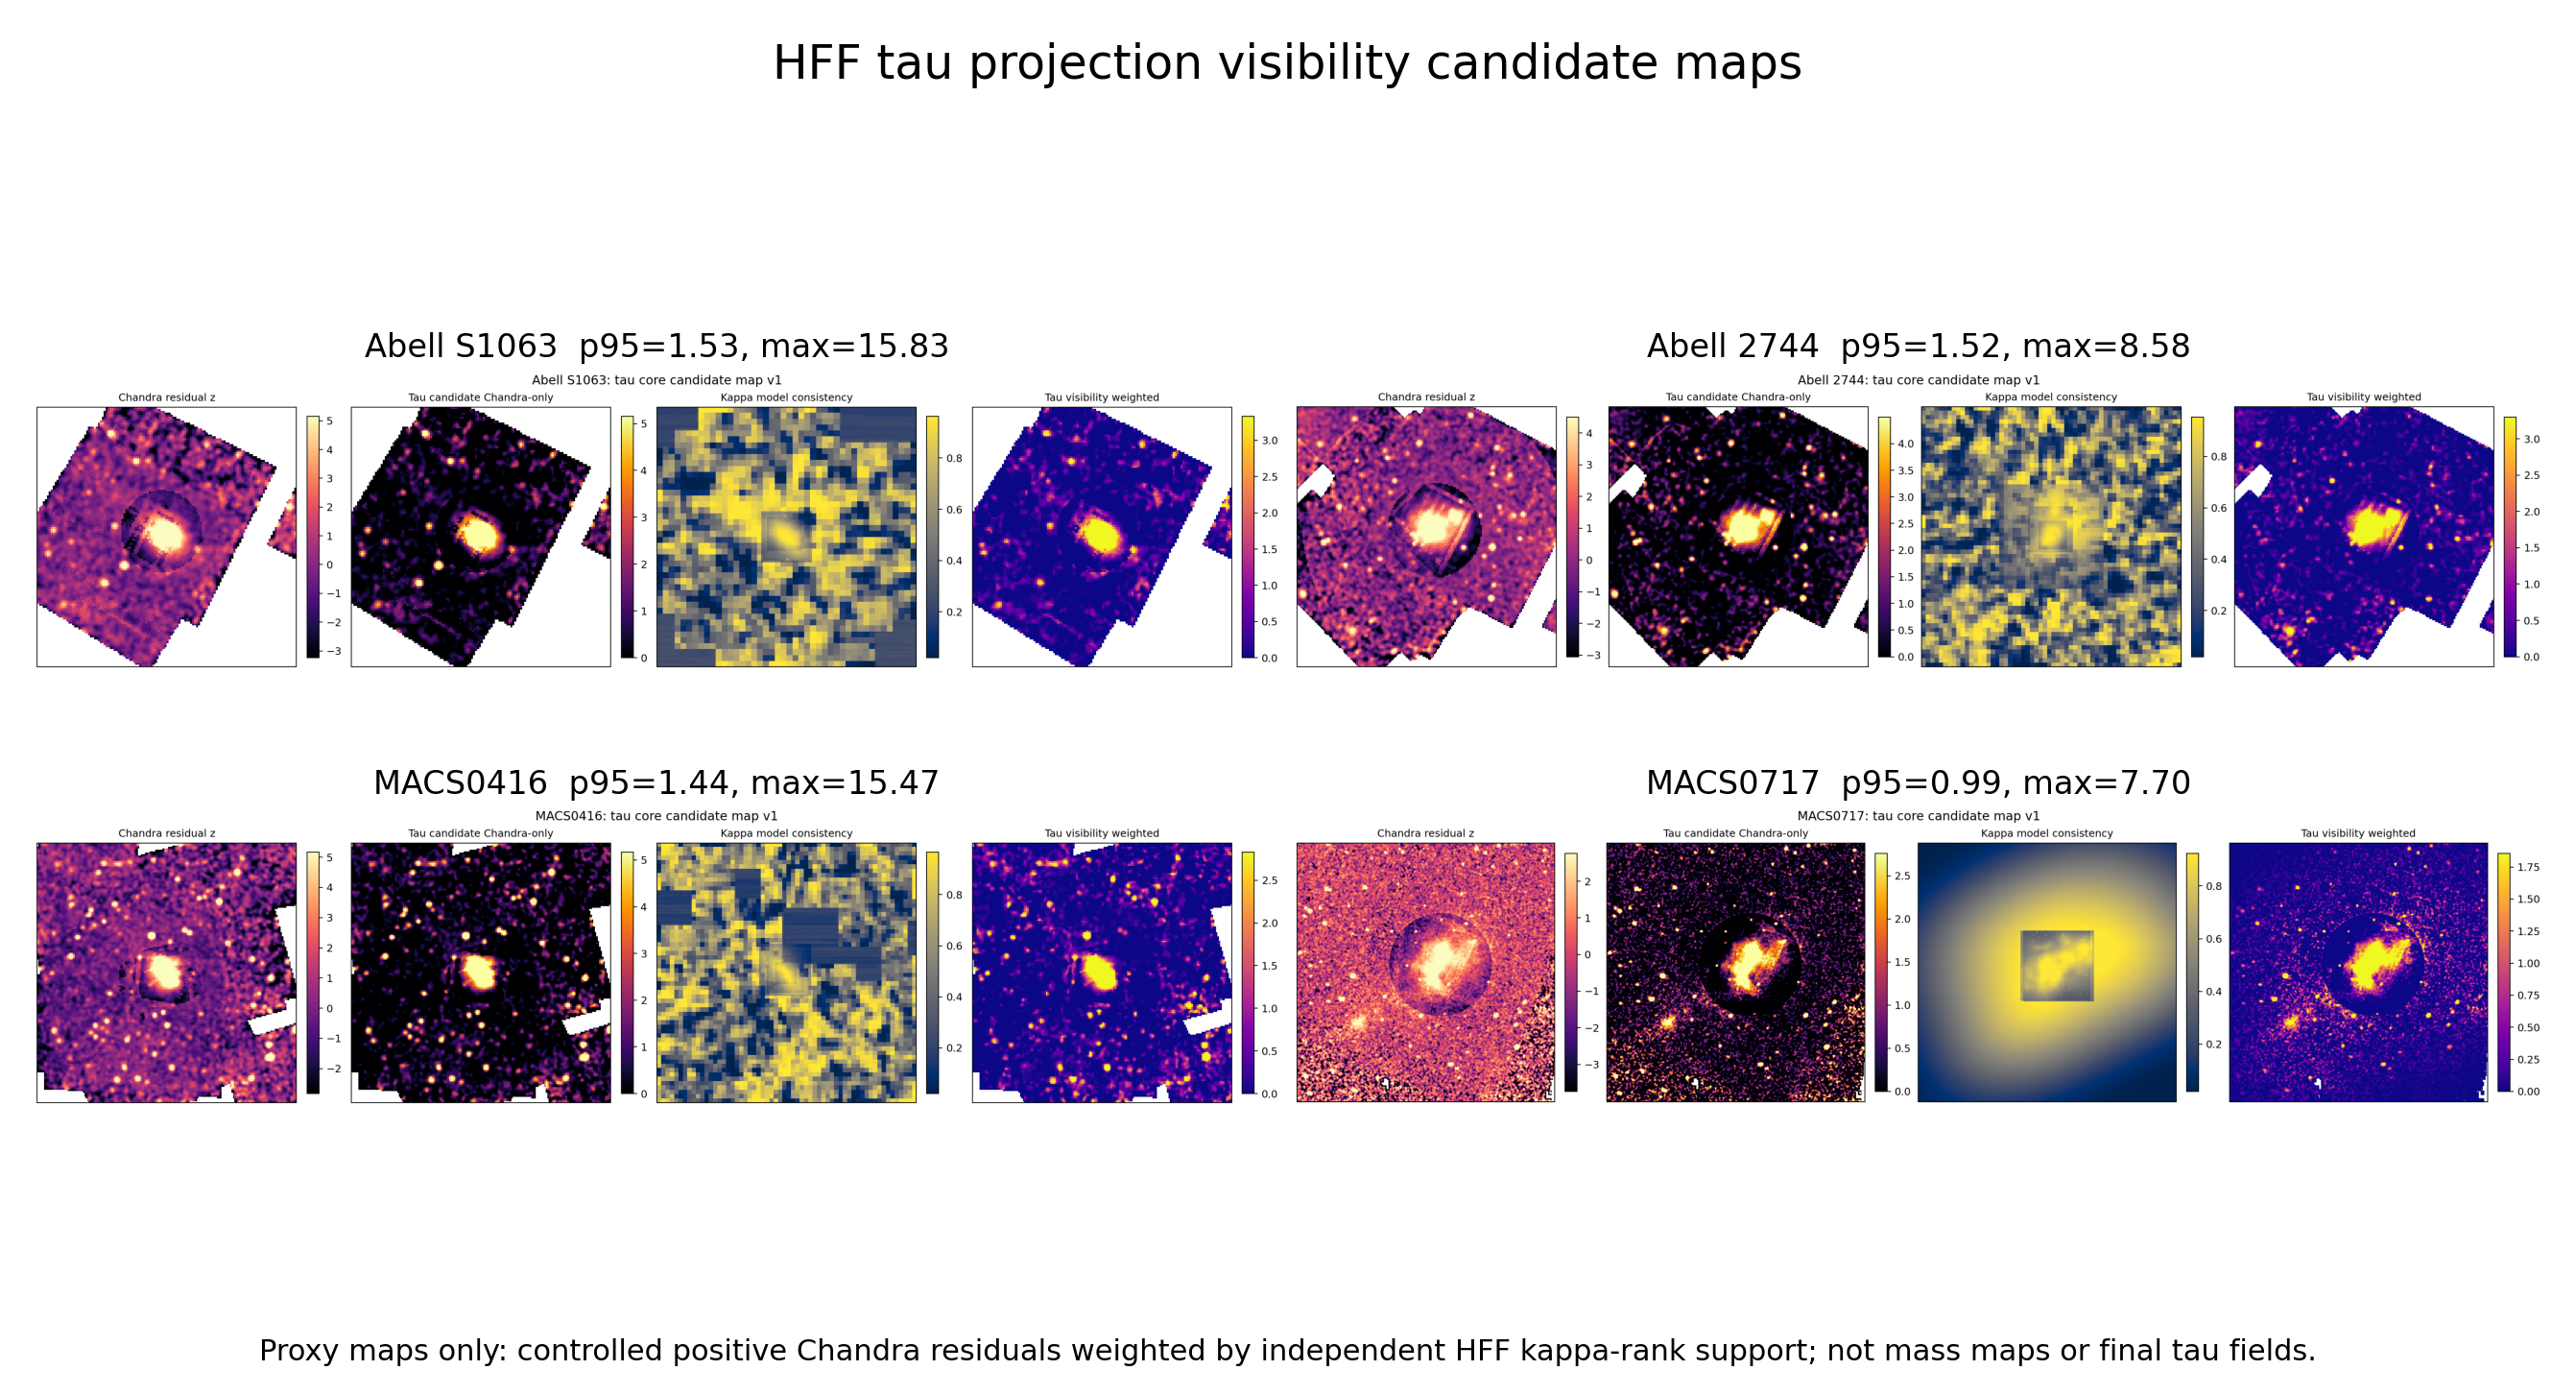
\includegraphics[width=0.98\textwidth]{figures/candidate_tau_visibility_maps_panel_v1.png}
\caption{Candidate visibility maps for the original four \HFF{} clusters. The
displayed field is not a mass map, a final physical field, or a derived
mechanism. It is a controlled
positive \Chandra{} residual weighted by the percentile-rank support of
independent \HFF{} convergence maps.}
\label{fig:candidate-maps}
\end{figure}

\section{Interpretation and Scope}

The current result supports an exploratory cross-readout enrichment result:
\begin{quote}
controlled X-ray residual geometry is usually enriched inside high
lensing-readout regions above matched nulls.
\end{quote}
It does not support a universal lensing-readout claim, because Abell 370 and
MACS0717 retain below-null magnification channels. It also does not require
introducing a hidden component inside the observational statistic. The allowed
interpretation in this paper is deliberately conservative: a controlled
phenomenological enrichment statistic in cluster lensing. The disallowed
interpretation is a renamed hidden density or a derived new-gravity mechanism.

Projection-based frameworks, including \(\tau\)-core-like interpretations, may
treat this prefilter as an empirical constraint. They are not part of the
paper's central claim. In particular, this paper does not provide a dynamical
equation, action, field equation, relativistic consistency proof, lensing
derivation, or covariant structure. Those belong to a separate theory paper.

\section{Falsification Criteria}

The branch would fail if:
\begin{enumerate}[leftmargin=*]
\item the signal disappears under radius/exposure controls;
\item the signal is reproduced by roll or value-shuffle controls;
\item the signal depends on a single model family;
\item the analysis switches from magnification to convergence only after seeing
the data;
\item a proposed physical interpretation predicts all Abell 370 or MACS0717 lensing products
are positive.
\end{enumerate}
The last condition is already active: Abell 370 and MACS0717 magnification
failures forbid the strongest universal version of the claim.

\section{External Blind Protocol}

The next sample-expansion branch should be run under a frozen protocol. Before
examining the enrichment outcome for any new cluster sample, the analysis must
declare the cluster list, admissible model families, observable channels,
primary tracer, compact-source mask, enrichment metric, top-region thresholds,
null families, primary endpoint, secondary endpoints, and failure criteria.
The primary unit should be the cluster, not the pixel or model/observable row.
The primary endpoint should be the cluster median residual/null ratio across
predeclared admissible rows. Kappa and magnification must remain separate
channels, and a below-null channel must stay in the table rather than being
replaced by a stronger observable after inspection.

This blind protocol is required before any population-level claim. In the
current branch it has been applied once to the external CLASH map-level sample.
The frozen external pass rule is that the spatial-block-aware hierarchical
population residual/null ratio must have a lower approximate 95 percent
interval above unity. This creates an external validation layer, while still
requiring broader public replication before a population-level astrophysical
claim.

\section{HFF All-Six Expansion Status}

The nearest homogeneous map-level expansion was to complete the two remaining
\HFF{} clusters, Abell 370 and MACS J1149.5+2223. In the current branch, the
public lensing side of that extension has been acquired and audited: Merten,
CATS, Diego, and Williams kappa and \(z=4\) magnification products are available
locally for both clusters, with README files, checksums, finite-pixel checks,
and WCS checks recorded in the acquisition manifest.

The \Chandra{} side now has first-pass uniform products for both systems. A
Chandra Data Archive TAP catalog query finds archived, no-grating observations
for both systems: Abell 370 has 104 archived observations totaling
\(1998.062\) ks, while MACS J1149.5+2223 has 8 archived observations totaling
\(365.425\) ks. Both stacks were processed through the local CIAO pipeline and
then through the common prefilter runner. This upgrades the branch from a
four-cluster pilot to an all-six first-pass \HFF{} audit, while retaining the
need for spatial-autocorrelation-aware uncertainty and formal cluster-level
meta-analysis before any population claim.

\section{External CLASH Map-Level Validation}

After the \HFF{} all-six audit, the branch froze a direct external CLASH
map-level validation run. The external runner does not pool CLASH with the
\HFF{} development rows. It repeats the same observational question on
independent public cluster systems, with declared CLASH model families,
declared lensing observables, declared \Chandra{} tracers, and the same
matched-null enrichment ratio.

The frozen CLASH run contains 96 model/observable/tracer rows across 12
clusters. Of these, 85 rows have residual/null ratio above unity. The row-level
median is 1.205, with a minimum of 0.453 and a maximum of 1.757. The weakest
rows are concentrated mainly in magnification plus residual-tracer channels,
so the external validation preserves the model-sensitivity already visible in
the \HFF{} development audit.

\begin{figure}[p]
\centering
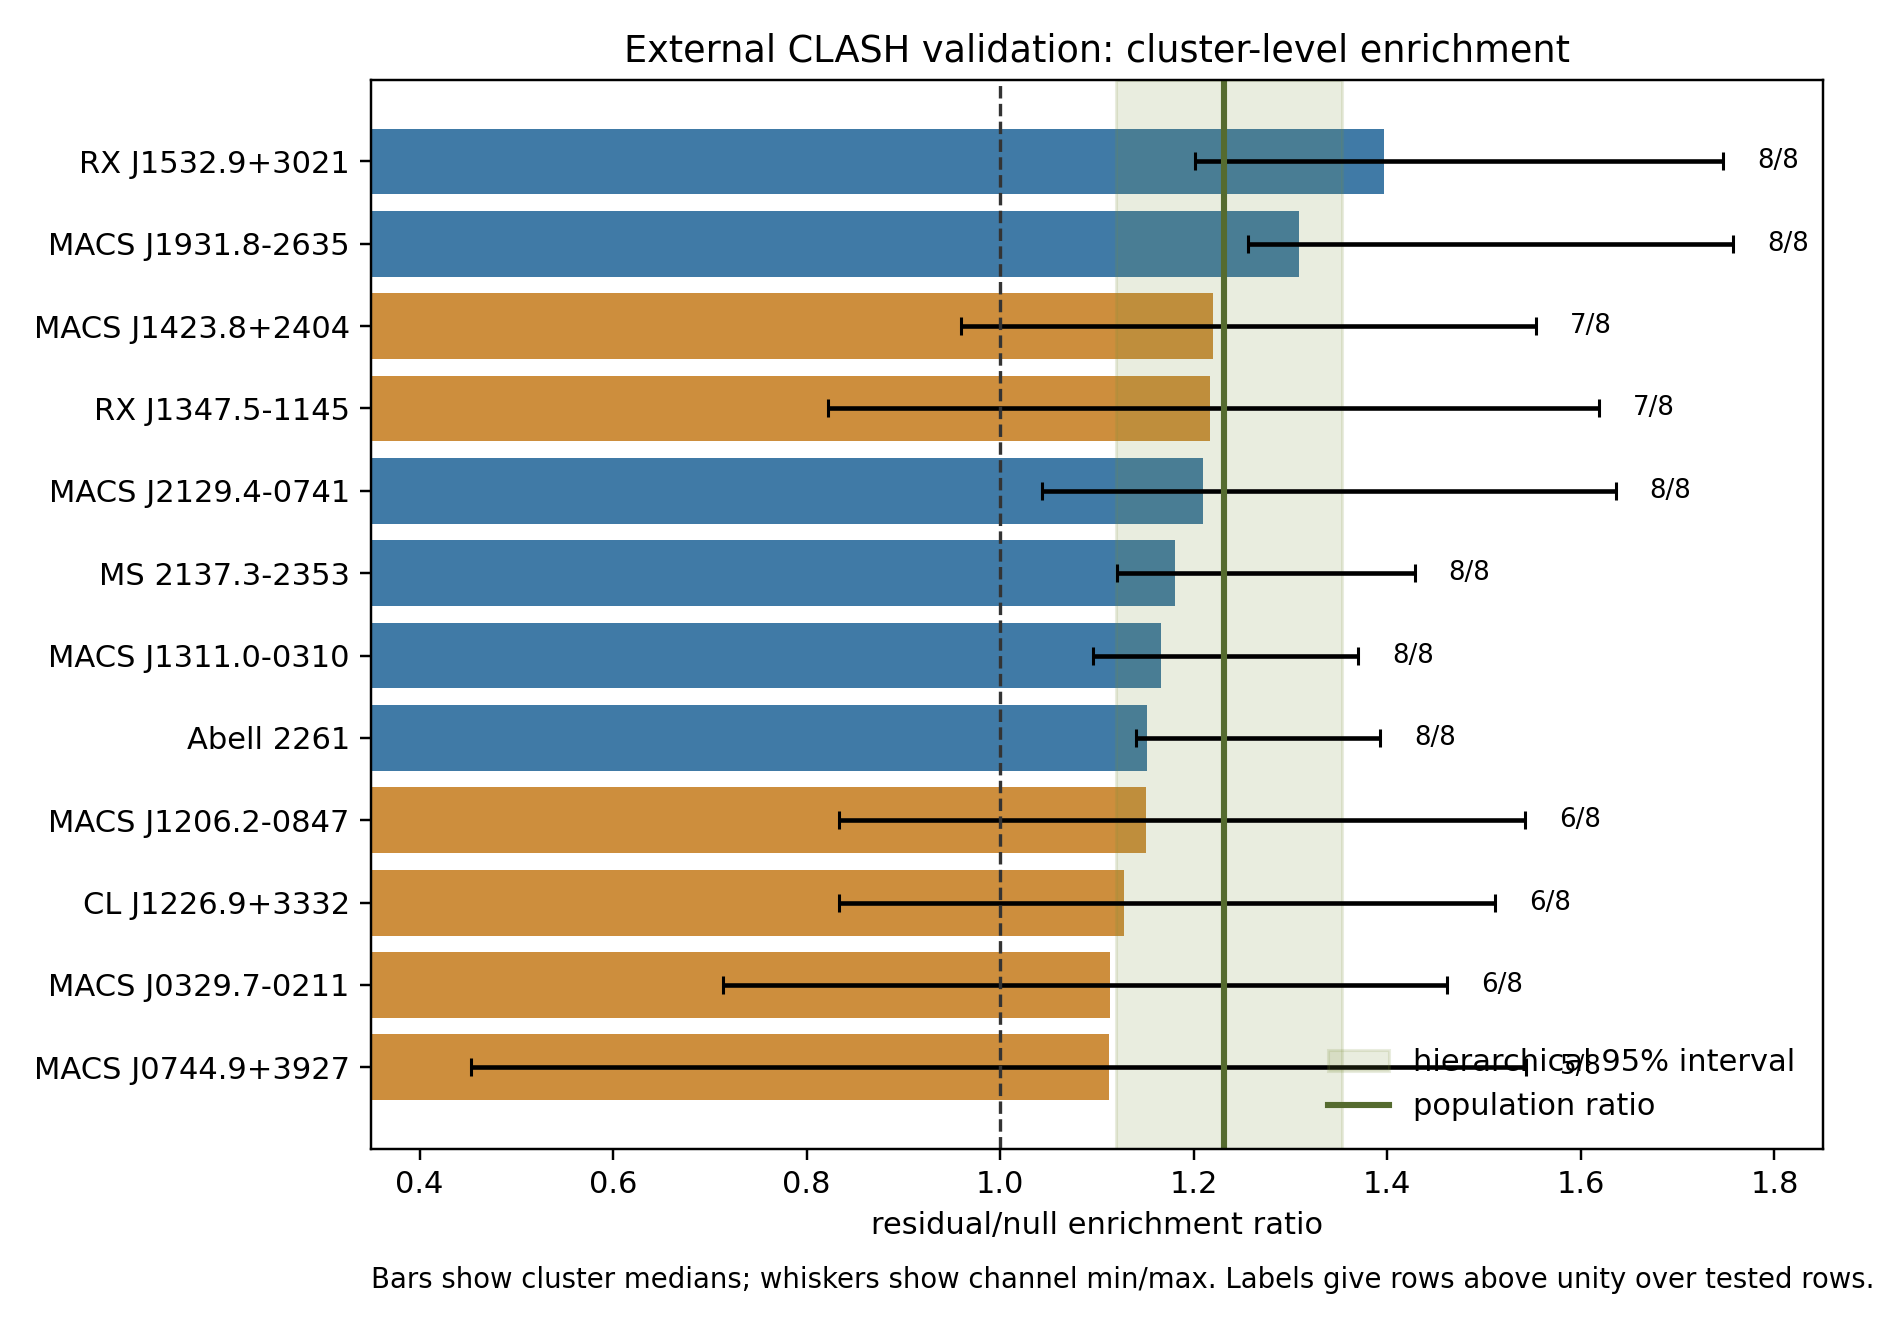
\includegraphics[width=0.92\textwidth]{figures/external_clash_cluster_validation_summary_v1.png}
\caption{External CLASH map-level validation. Bars show cluster-level median
residual/null enrichment ratios across the frozen Zitrin LTM-Gauss/NFW
kappa/magnification and \Chandra{} tracer rows; whiskers show the within-cluster
channel minimum and maximum. The shaded band shows the approximate 95 percent
hierarchical population interval, and the vertical green line shows the fitted
population ratio. Labels report rows above unity over tested rows.}
\label{fig:external-clash-cluster-validation}
\end{figure}

\begin{figure}[p]
\centering
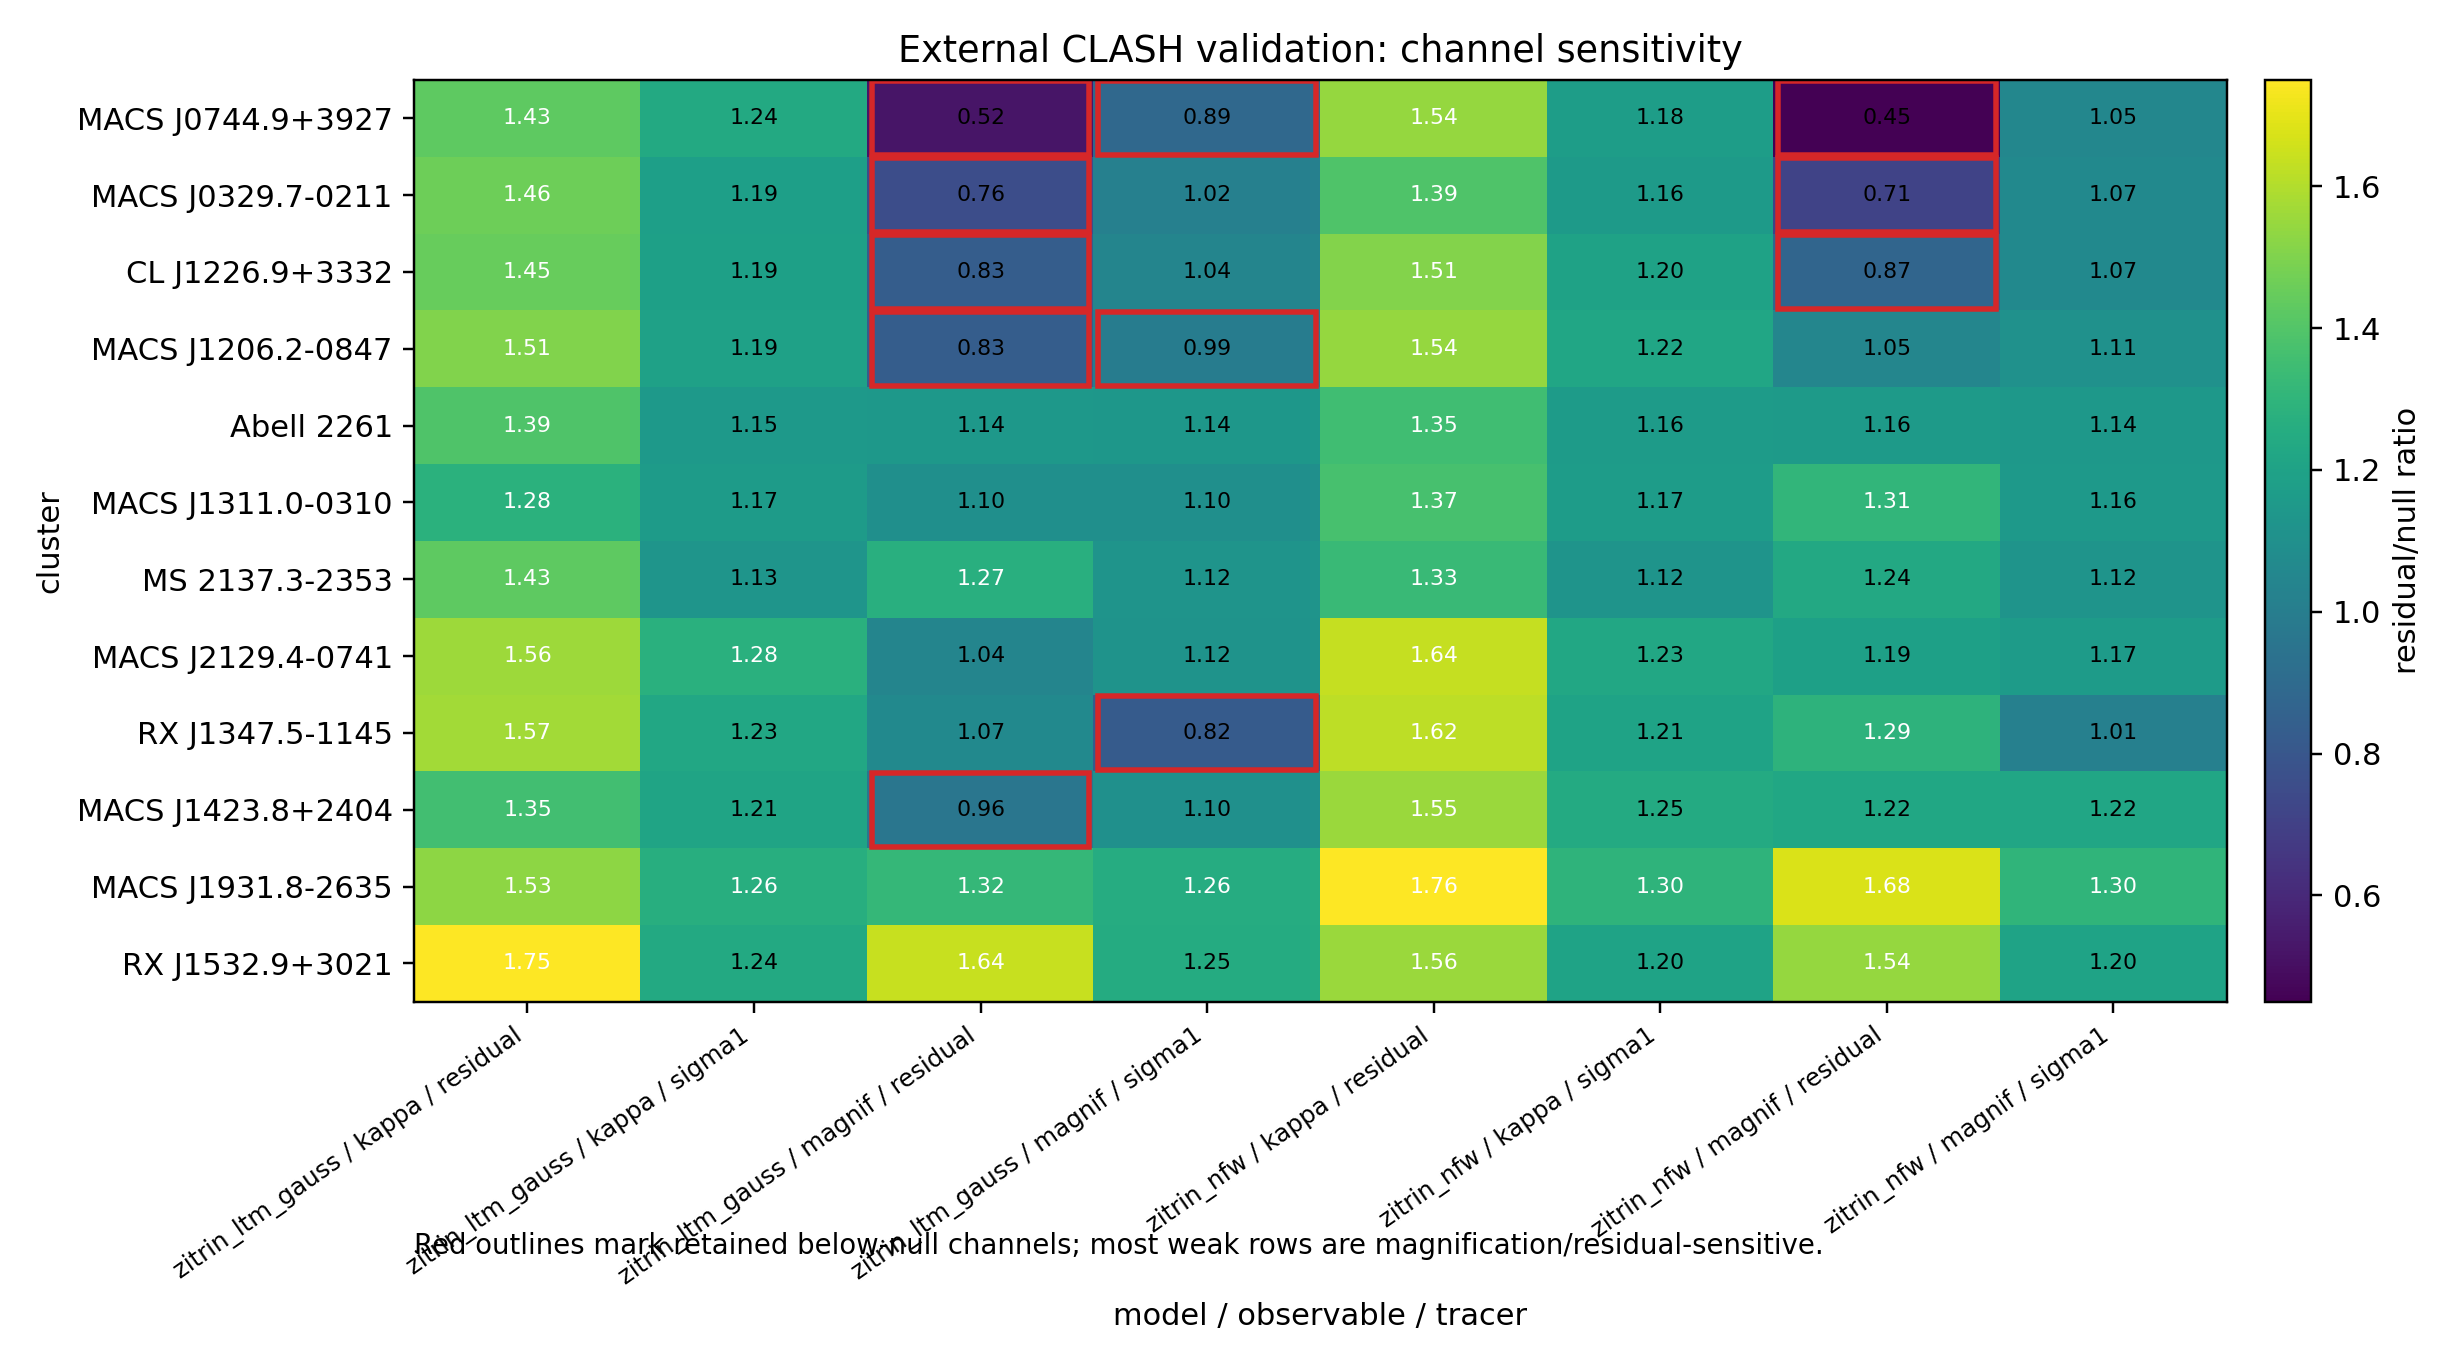
\includegraphics[width=0.98\textwidth]{figures/external_clash_channel_sensitivity_heatmap_v1.png}
\caption{External CLASH channel sensitivity. Each cell is the observed
enrichment divided by the matched-null mean for one frozen
cluster/model/observable/tracer row. Red outlines mark retained below-null
channels. The figure is intentionally not collapsed to a single positive
number: the external result passes at population level while preserving
magnification/tracer sensitivity as a real limitation.}
\label{fig:external-clash-channel-sensitivity}
\end{figure}

\begin{center}
\begin{tabular}{lr}
\toprule
Cluster & Median $R_{\mathrm{null}}$ \\
\midrule
MACS J0744.9+3927 & 1.113 \\
MACS J0329.7-0211 & 1.113 \\
CL J1226.9+3332 & 1.128 \\
MACS J1206.2-0847 & 1.150 \\
Abell 2261 & 1.152 \\
MACS J1311.0-0310 & 1.167 \\
MS 2137.3-2353 & 1.181 \\
MACS J2129.4-0741 & 1.210 \\
RX J1347.5-1145 & 1.217 \\
MACS J1423.8+2404 & 1.220 \\
MACS J1931.8-2635 & 1.309 \\
RX J1532.9+3021 & 1.397 \\
\bottomrule
\end{tabular}
\end{center}

Spatial-block bootstrap uncertainties were then propagated into an external
hierarchical fit with cluster and channel random intercepts. The fitted
population log-ratio is
\[
\hat{\mu}_{\mathrm{CLASH}}=0.208,
\]
corresponding to a population residual/null ratio of
\[
\exp(\hat{\mu}_{\mathrm{CLASH}})=1.231,
\]
with an approximate 95 percent interval of 1.119 to 1.353. The frozen external
pass criterion is therefore satisfied. The fitted variance components are
\[
\sigma_{\mathrm{cluster}}=0.076,\qquad
\sigma_{\mathrm{channel}}=0.118,\qquad
\sigma_{\mathrm{residual}}=0.026,
\]
with median spatial-block log uncertainty 0.103.

This is stronger than the earlier proxy-level CLASH check because it uses
actual map-level lensing/X-ray co-structure. It is still not a mechanism
derivation and not a hidden-mass claim. The paper-safe reading is narrower:
the same controlled cross-readout enrichment statistic that was developed on
\HFF{} clusters also passes a frozen external map-level CLASH validation.

\section{Reproducibility Layer}

The current branch now has an internal open-science scaffold. The frozen
protocol YAML freezes the random seed, top-region thresholds, matched-null
count, negative-control count, radius/exposure binning, compact-source mask,
primary endpoint, secondary endpoints, and failure rules. A release manifest
lists the protocol file, paper source, runner scripts, validators, generated
tables, and figures that should be released together. The exact local files are
the protocol YAML and reproducibility manifest listed in the project README and
readiness ledger.

This does not yet make the branch fully public-reproducible. A public package
still needs source-data download scripts, released masks, exact source-data
metadata, final license/citation text, and one-command reproduction
instructions. The protocol file is therefore an internal freeze for the present
branch and a template for the prospective homogeneous sample expansion.

\section{First-Pass Hierarchical Meta-Analysis}

We fit a first-pass hierarchical model to the all-six \HFF{} runner table. The
response is
\[
\log R_{ij} =
\log\left(E_{\mathrm{obs},ij}/\langle E_{\mathrm{null},ij}\rangle\right),
\]
with a population intercept, cluster random intercepts, model/channel random
intercepts, and a residual term:
\[
\log R_{ij} = \mu + a_{\mathrm{cluster}[i]} + b_{\mathrm{channel}[j]} +
\epsilon_{ij}.
\]
The spatial-block-aware fitted population mean is positive:
\[
\hat{\mu}=0.489,\qquad
\exp(\hat{\mu})=1.630,
\]
with an approximate 95 percent interval of \(1.429\) to \(1.860\) on the
population residual/null ratio. The fitted variance components are
\[
\sigma_{\mathrm{cluster}}=0.091,\qquad
\sigma_{\mathrm{channel}}=0.246,\qquad
\sigma_{\mathrm{residual}}=0.161.
\]
The median spatial-block log uncertainty supplied to the fit is 0.114, with a
maximum of 0.537.

A correlation-length calibration estimates the \(1/e\) autocorrelation length
of the X-ray tracer maps. The median estimated correlation length is 102 native
pixels, with a 90th percentile of 225 pixels; the smoothed X-ray
\(\sigma_1\) maps have the longest tails. A block-size sensitivity sweep with
target block-axis counts of 4, 6, 8, 12, 16, 24, and 32 gives stable population
residual/null ratios from 1.611 to 1.633. This reduces the risk that the fitted
population effect is an artifact of one arbitrary spatial grid, while retaining
the caveat that very smooth tracer maps require conservative block choices.

This fit is useful because it quantifies a point already visible in the
descriptive tables: channel variation is larger than cluster variation. The
weakness is therefore not that whole clusters fail the audit, but that some
lensing/readout channels, especially magnification channels, sit below the
all-six pattern.

This is a real hierarchical fit with row-level spatial-block uncertainty, but
it remains a development-sample fit. The external CLASH map-level analysis now
provides the first frozen validation layer and should be reported separately
from the \HFF{} development rows. The two samples should not be pooled in one
undifferentiated model until a broader, predeclared multi-sample hierarchy is
specified.

\section{Limitations}

This draft is not submission-ready. The model-team README audit,
method-family BibTeX key coverage, compact-source masking audit, and
model-family uncertainty layer are complete at the current preprint-draft
level. Remaining blockers are narrower: the bibliography still needs final
publisher/ADS metadata verification; the \HFF{} development sample remains
small and \HFF{}-selected, with only six clusters; the two newly reduced
\HFF{} clusters are first-pass products; the CLASH external validation uses
one public model-team family in two parameterizations and therefore does not
replace broader multi-team external lens-model validation; MACS0717 has the
strongest compact-source radial-null layer while the other clusters currently
use enrichment-comparison masking audits; the first-pass random-effects
meta-analysis now includes spatial-block row uncertainties, block-size sweep,
correlation-length calibration, and one frozen external CLASH application, but
the rule should still be preregistered and repeated on broader samples; the
public reproducibility package is scaffolded but not yet released; the
rotation-curve branch remains separate; and any projection-based physical
interpretation, including \(\tau\)-core-like interpretations, remains a later
theory object until derived from explicit dynamical assumptions.

\section{Conclusion}

The \HFF{} plus external CLASH branch supports a paper-worthy observational
prefilter:
\begin{quote}
controlled lensing/X-ray cross-readout enrichment is detectable as a
model-sensitive spatial statistic in cluster lensing.
\end{quote}
The correct claim is deliberately narrow: a falsifiable, map-level
cluster-lensing enrichment statistic now survives both a \HFF{} development
audit and a frozen external CLASH validation. Its main value is as an empirical
phenomenology and as a constraint on later physical interpretations, not as a
derivation of such an interpretation.

\bibliographystyle{plainnat}
\bibliography{refs}

\end{document}
